\documentclass[letterpaper,12pt]{book}

\usepackage[utf8]{inputenc} % Soporte para acentos
\usepackage[T1]{fontenc}    
\usepackage[spanish,mexico]{babel} % Español

% Soporte de símbolos adicionales (matemáticas)
\usepackage{amsmath}		
\usepackage{amssymb}		
\usepackage{amsfonts}
\usepackage{latexsym}

% Para inserción de imagenes
\usepackage[pdftex]{graphicx}

% Para crear bibliografía por capítulo o sección
\usepackage[globalcitecopy]{bibunits}
% Para este paquete el proceso de compilación se llevará a cabo de la siguiente forma:
% - pdflatex
% - bibtex
% Por cada entorno bibunit se crearán archivos bu1.aux, bu2.aux, ...
% Para cada uno de estos archivos se debe ejecutar el comando:
% - bibtex bu1.aux
% - bibtex bu2.aux
% ... a continuación:
% - pdflatex
% - pdflatex

\usepackage[lmargin=2cm,rmargin=2cm,top=2cm,bottom=2cm]{geometry}

% Información para el título
\title{Notas al Pie \\ 
	\vspace{1cm}Tablas de Contenidos \\ 
	\vspace{1cm}Índice de Figuras y Tablas\\
	\vspace{1cm}Bibliografía}
\author{J. Luis Torres}

% Indicamos una separación entre los párrafos
\parskip=3mm

% Eliminamos la sangría de los párrafos
\parindent=0mm

\bibliographystyle{apalike}

% El siguiente bloque es necesario para que la bibliografía en los capítulos se genere
% con una estructura de sección. De lo contrario se colocará siempre en una página nueva.
\let\stdthebibliography\thebibliography
\renewcommand{\thebibliography}{%
\let\chapter\subsection
\stdthebibliography}


\newcommand{\tituloTesis}[1]{\def\eltituloTesis{#1}}
\newcommand{\titulo}[1]{\def\elTitulo{#1}}
\newcommand{\nombre}[1]{\def\elnombre{#1}}    %* Del alumno
\newcommand{\appat}[1]{\def\elApPaterno{#1}}    %* Del alumno
\newcommand{\apmat}[1]{\def\elApMaterno{#1}}    %* Del alumno
\newcommand{\director}[1]{\def\eldirector{#1}}  %* De tesis
\newcommand{\fecha}[1]{\def\lafecha{#1}}
\newcommand{\logoUNAM}[1]{\def\ellogoUNAM{#1}}
\newcommand{\logoCiencias}[1]{\def\ellogoCiencias{#1}}

\newenvironment{changemargin}[2]{% 
\begin{list}{}{% 
\setlength{\topsep}{20pt}% 
\setlength{\leftmargin}{#1}% 
\setlength{\rightmargin}{#2}% 
}% 
\item[]}{\end{list}} 

\logoUNAM{unam}%Nombre de la imagen que contiene el escudo de la UNAM
\logoCiencias{ciencias}
\tituloTesis{TEOREMA DE LAMPORT}
\nombre{JESUS}
\appat{SANCHEZ}
\apmat{ALCANTARA}
\titulo{COMPU} %Titulo que voy a obtener
\director{DR.PANCHO LOPEZ} 
\fecha{\the\year}

\begin{document}

\begin{changemargin}{0cm}{0cm}
%%%%%%%%%%%%%%%%%%%%%%%%%%%%%%%%%%%%%%%%%%%%%%%%%%%%%%%
%% Comandos para la portada
\thispagestyle{empty}
\begin{center}
%% Barra izquierda - Escudos
\hskip-1cm
\vskip1.5cm
\begin{minipage}[c][14cm][s]{0.2\textwidth} 
  \begin{center}
    \includegraphics[width=0.8\textwidth]{\ellogoUNAM}\\[10pt] % Escudo de la UNAM.
    \hskip2pt\vrule width2pt height13cm\hskip1mm
    \vrule width1pt height13cm\\[10pt]
    \includegraphics[width=0.8\textwidth]{\ellogoCiencias} % Escudo de Ciencias
  \end{center}
\end{minipage} \quad
%% Barra derecha - Tí­tulos
\begin{minipage}[c][14cm][s]{0.7\textwidth}
  \begin{center}
    % Barra superior
    {\Large \scshape Universidad Nacional Aut\'onoma de M\'exico}
    \vspace{.3cm}
    \hrule height2pt
    \vspace{.1cm}
    \hrule height1pt
    \vspace{.3cm}
    {\scshape \large Facultad de Ciencias}

    % Titulo del trabajo
    \vspace{3cm}

    {\huge \scshape \rmfamily \eltituloTesis} %Los primeros tres son para el formato del texto del titulo de la tesis (modificables a gusto)

    \vspace{3cm}

    % Tipo de trabajo
    \makebox[0.7\textwidth][s]{\huge T E S I S}\\[25pt]
    \makebox[0.7\textwidth][s]{QUE PARA OBTENER EL T\'ITULO DE:}\\[10pt]
    \begin{center}{\scshape \large \elTitulo}\end{center}%\\[13pt]
    \makebox[0.7\textwidth][s]{P R E S E N T A:}\\[10pt]
    \begin{center}{{\scshape \elnombre} \hspace{2ex} {\scshape \elApPaterno} \hspace{2ex} {\scshape \elApMaterno}}\end{center}

    \vspace{1.5cm}

    {\small DIRECTOR DE TESIS:\\ \uppercase{\eldirector}}

    \vspace{1cm}

    \lafecha
    
  \end{center}
\end{minipage}
\end{center}
\end{changemargin}


\maketitle

\tableofcontents


\chapter{Gráficas sencillas con Maple 15}
%Entorno para indicar la unidad bibliografica que va a utilizar[estilo de bibliografía]
\begin{bibunit}[plain]

\emph{Maple} es considerado un \emph{Sistema de Álgebra Computacional}, proporciona múltiples
funcionalidades al usuario entre las que se pueden listar las siguientes:

Las siguientes instrucciones nos permiten definir una función y generar su gráfica 
em Maple 15:

\begin{verbatim}
k:= x -> sin(x) + exp(cos(exp(x)));

plot(k(x), x=-10..4.5);
\end{verbatim}

Estas instrucciones nos permiten generar la gráfica que se muestra en la figura \ref{cap1f1}.

\begin{figure}[h!]
\centering
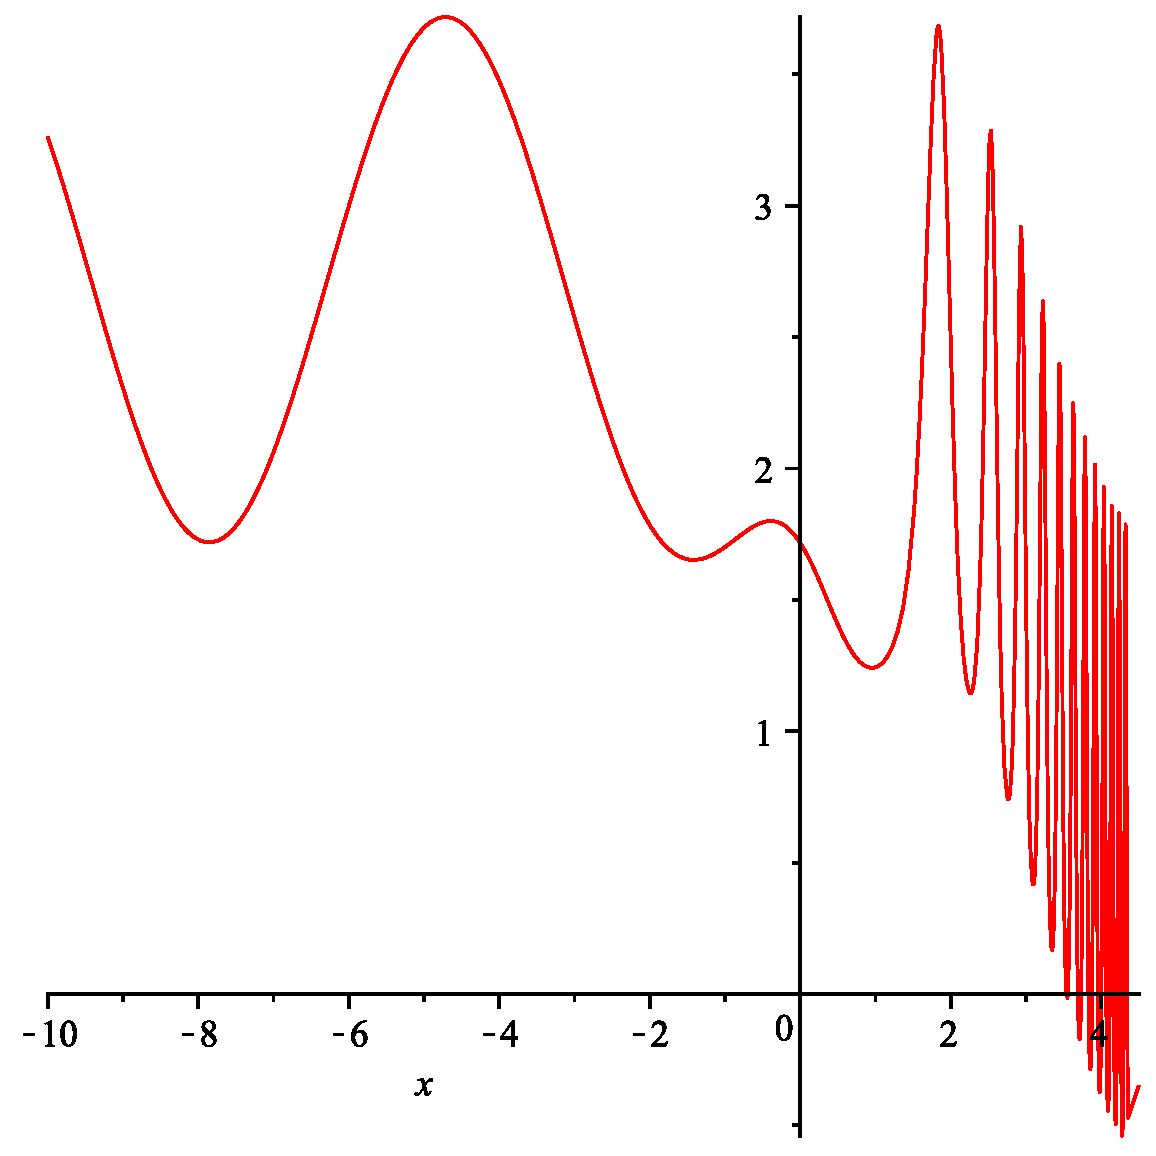
\includegraphics[scale=0.45]{grafica01}
\caption{Gráfica de $sen \left( x \right) +{{\rm e}^{\cos \left( {{\rm e}^{x}} \right) }}$}\label{cap1f1}
\end{figure}

\pagebreak

Veamos otro ejemplo:

Las siguientes instrucciones nos permiten generar la gráfica de la función 
$\displaystyle {x}^{4}\sin \left( {x}^{3} \right) -{x}^{3}\cos \left( {x}^{2}
 \right) +{x}^{2}\sin \left( x \right) -x$

\begin{verbatim}
plot(x^4*sin(x^3)-x^3*cos(x^2)+x^2*sin(x)-x, x = -1.8 .. 1.8);
\end{verbatim}

La gráfica se muestra en la figura \ref{cap1f2}.

\begin{figure}[h!]
\centering
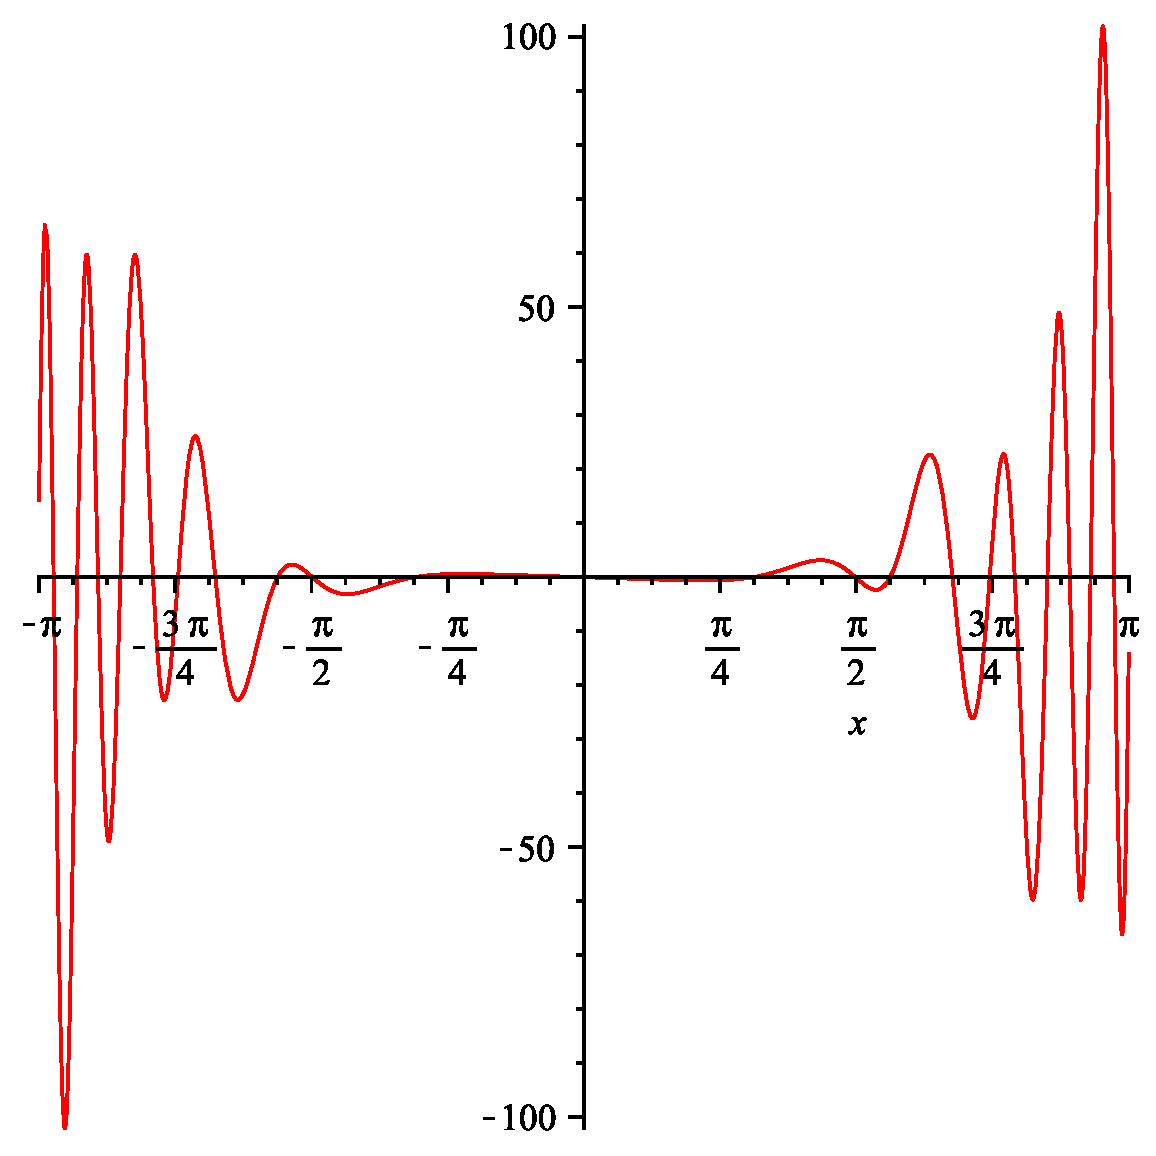
\includegraphics[scale=0.5]{grafica02}
\caption{Gráfica de ${x}^{4}\sin \left( {x}^{3} \right) -{x}^{3}\cos \left( {x}^{2}
 \right) +{x}^{2}\sin \left( x \right) -x$}\label{cap1f2}
\end{figure}

En la tabla \ref{tab:cap1t1} podemos consultar algunas instrucciones de \emph{Maple} que nos
permiten generar gráficas en dos dimensiones. \cite{Lamport}

\begin{table}[h!]
	\caption{Instrucciones de Maple para gráficas en 2D}
	\begin{center}
		\begin{tabular}{|c|c|} \hline
			Instrucción & Tipo de gráfica generada \\ \hline
			plot() & Gráficas en 2D de funciones explicitas \\ \hline
			plot() & Gráficas en 2D de funciones paramétricas \\ \hline
			polarplot() & Gráficas en coordenadas polares \\ \hline
			implicitplot() & Gráficas implícitas en 2D \\ \hline
			complexplot() & Gráficas de expresiones complejas \\ \hline
			contourplot & Gráficas de contornos \\\hline
		\end{tabular}
	\end{center}
	\label{tab:cap1t1}
\end{table}

%Lugar donde va a colocar la bibliografía con putbib[nombreArchivo(s)]
\putbib[mibiblio]
%\addcontentsline{toc}{section}{Bibliografía Cap.1}

\end{bibunit}



\chapter{Gráficas de Funciones con Discontinuidades}
\chaptermark{Gráficas con Discontinuidades}

\begin{bibunit}[plain]

Para poder generar gráficas de funciones de este tipo, la opción
\emph{discont=true} nos permite indicar a \emph{Maple} que éstas deben eliminarse de la
gráfica. La forma en la que incluimos esta opción es la siguiente:

\begin{verbatim}
plot(funcion(x), x = intervalo, {rango}, discont = true);
\end{verbatim}

Por ejemplo, la siguiente instrucción nos permite desplegar una gráfica de la 
función \emph{tan(x)}:

\begin{verbatim}
plot(tan(x), x = -10 .. 10, -50 .. 50, discont = true);
\end{verbatim}

La gráfica se puede ver en la figura \ref{cap2f1}.

\begin{figure}[h!]
\centering
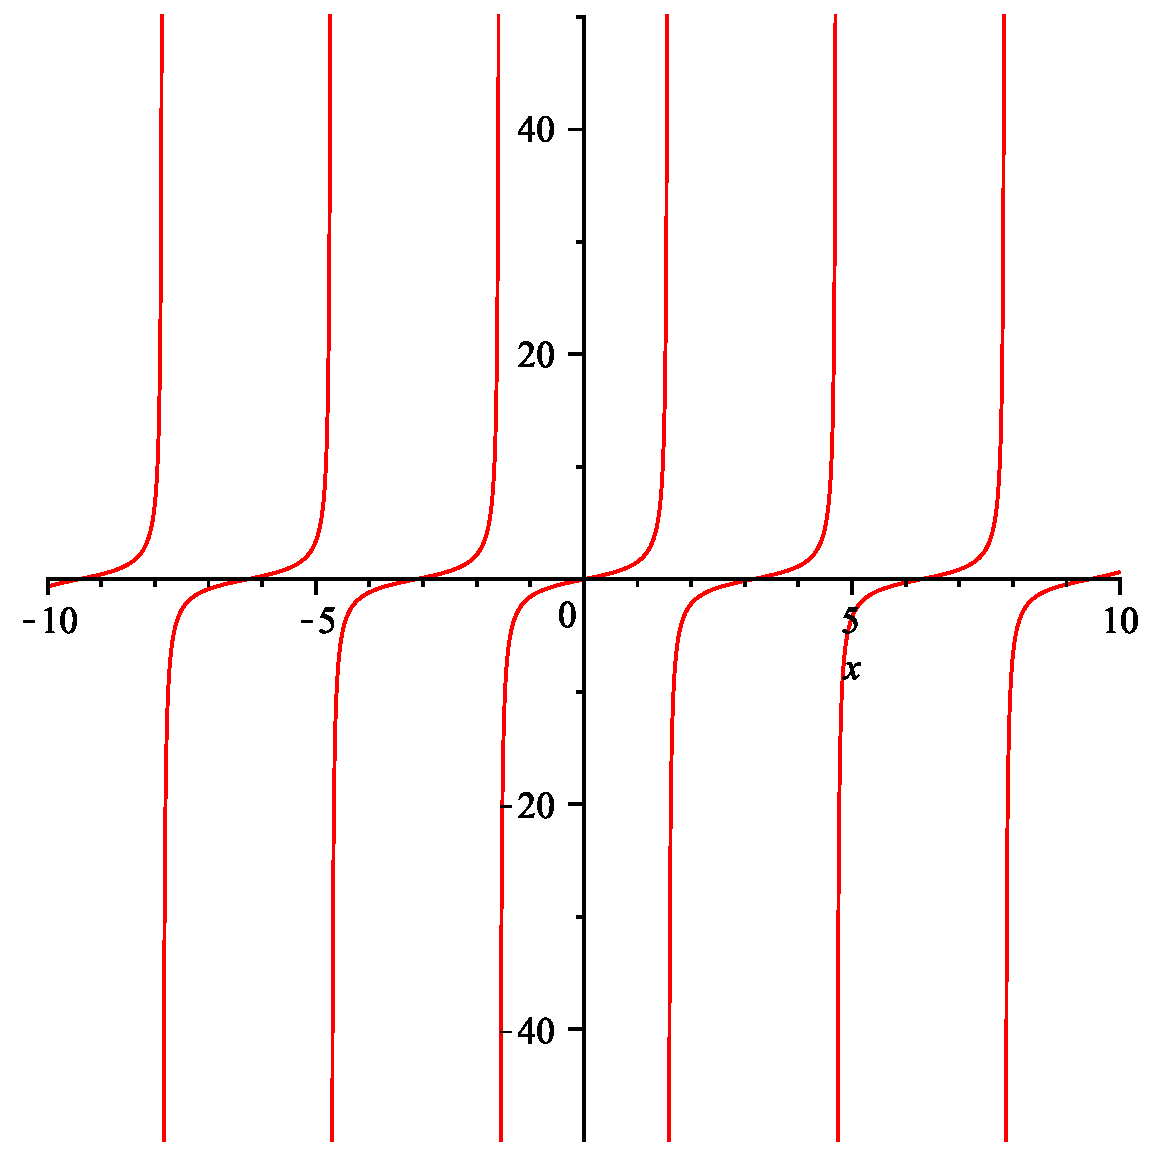
\includegraphics[scale=0.4]{grafica04}
\caption{Gráfica de $tan (x)$}\label{cap2f1}
\end{figure}

Consulte \cite[cap. 2]{spivakCalc} para aprender algo de límites.

\LaTeX{} es un sistema para la composición de documentos \cite[cap. ~2]{Lamport} para aprender algo de \LaTeX{}.

\putbib[mibiblio]

\end{bibunit}



\chapter{Gráficas con Múltiples Funciones}

La siguiente instrucción nos permite incluir las gráficas de varias funciones en un mismo despliegue:

\begin{verbatim}
plot({x, cos(x), sin(x)}, x, color = [blue, brown, green]);
\end{verbatim}

La gráfica se puede observar en la figura \ref{cap3f1}.

\begin{figure}[h!]
\centering
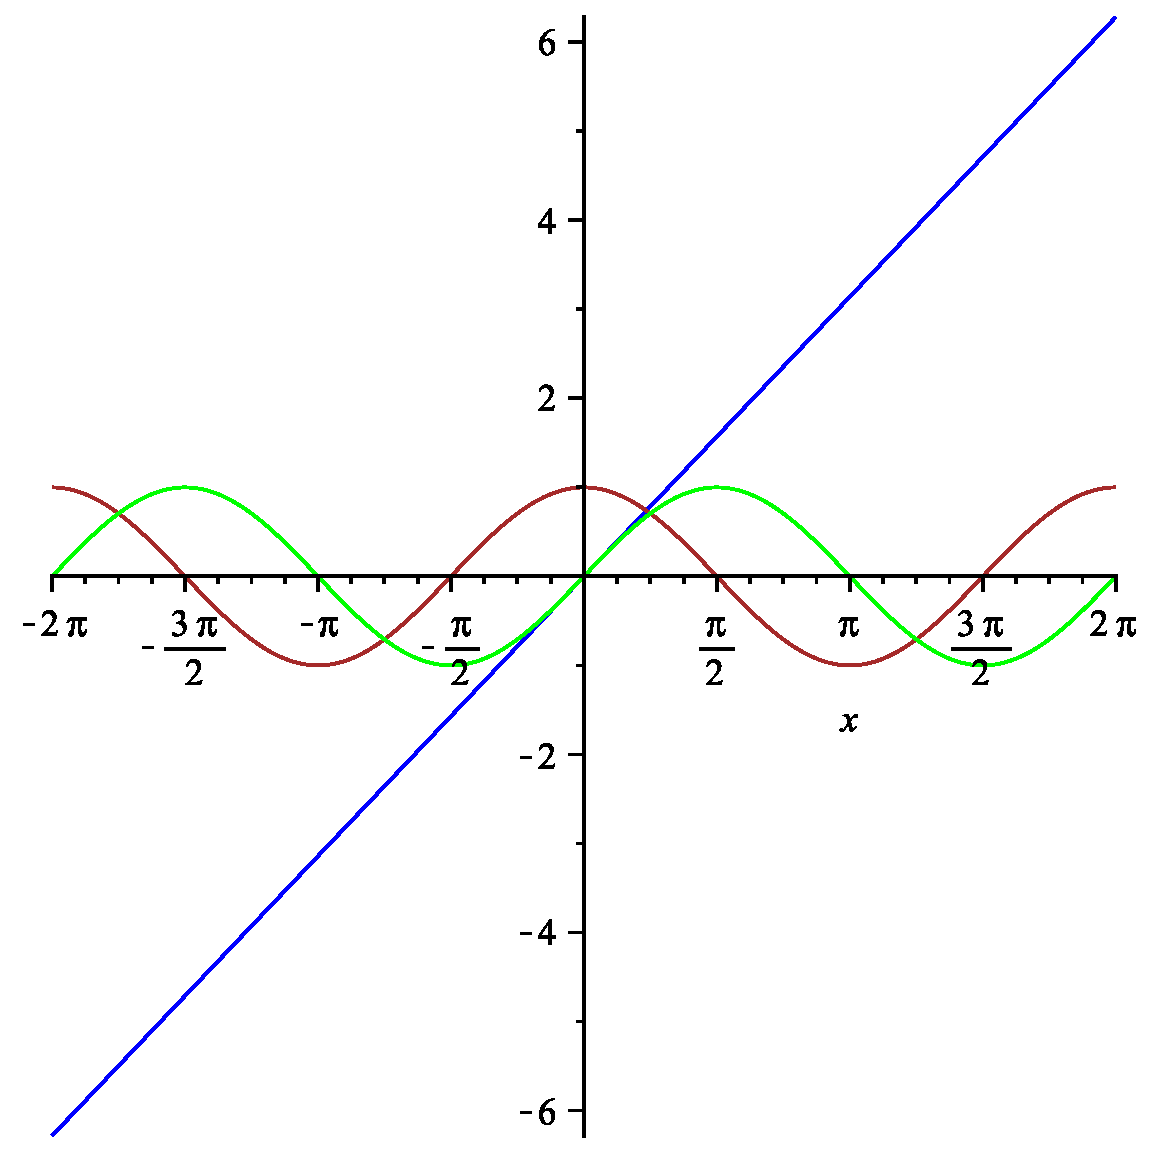
\includegraphics[scale=0.35]{grafica05}
\caption{Gráficas de $x$, $cos(x)$ y $sen(x)$}\label{cap3f1}
\end{figure}



\chapter[Apendice A. Bib\TeX{}]{Bib\TeX{}}

\section{Propiedades soportadas}

Algunas de las propiedades soportadas por Bib\TeX{} son:

\begin{tabular}{llll}
address & abstract & author & booktitle \\
chapter & contents & copyright & crossref \\
edition & editor & howpublished & institution \\
ISBN & ISSN & journal & key \\
keywords & language & month & note \\
number & organization & pages & publisher \\
school & series & title &url \\
volume & year & & 
\end{tabular}

\newpage

\section{Tipos de citas}

Algunos de los tipos de citas válidos en los archivos de 
\emph{bases de datos} de Bib\TeX{} son:

\begin{tabular}{lll}
article & book & booklet \\
conference & inbook & incollection \\
inproceedings & manual & mastersthesis \\
misc & other & phdthesis \\
proceedings & techreport & unpublished
\end{tabular}


%\putbib[mibiblio]
\bibliography{mibiblio}
\addcontentsline{toc}{chapter}{Bibliografía}

\end{document}
